\clearpage
\setcounter{page}{1}

\section{Langkah Kerja}
\begin{enumerate}

\item Pertama buka oracle apex, jika belum memiliki akun maka klik get started for free\\
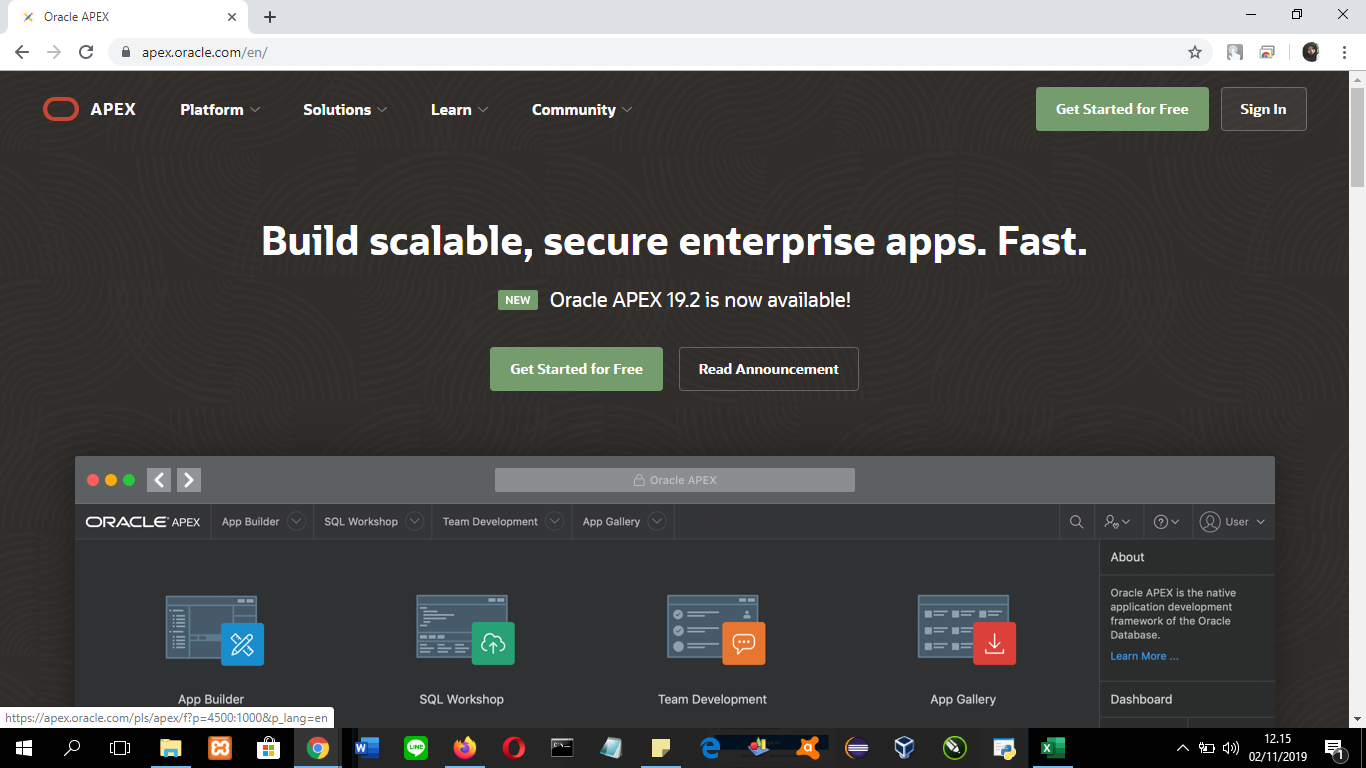
\includegraphics[scale= 0.3]{gambar/gambar1.png}\\
Klik request a free workspace\\
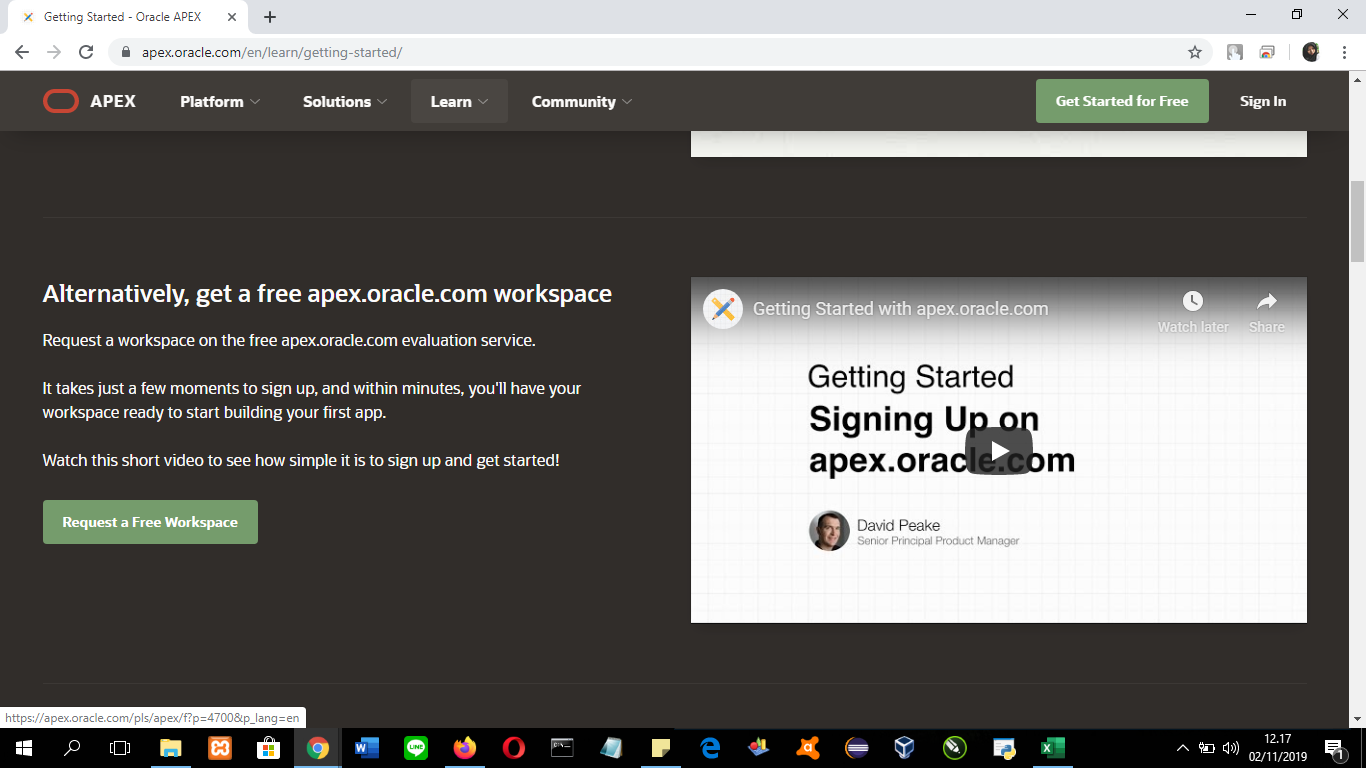
\includegraphics[scale= 0.3]{gambar/gambar2.png}\\
Lalu isi sesuai dengan data hingga step selesai.\\
Jika kalian sudah memiliki akun, maka klik sign in\\
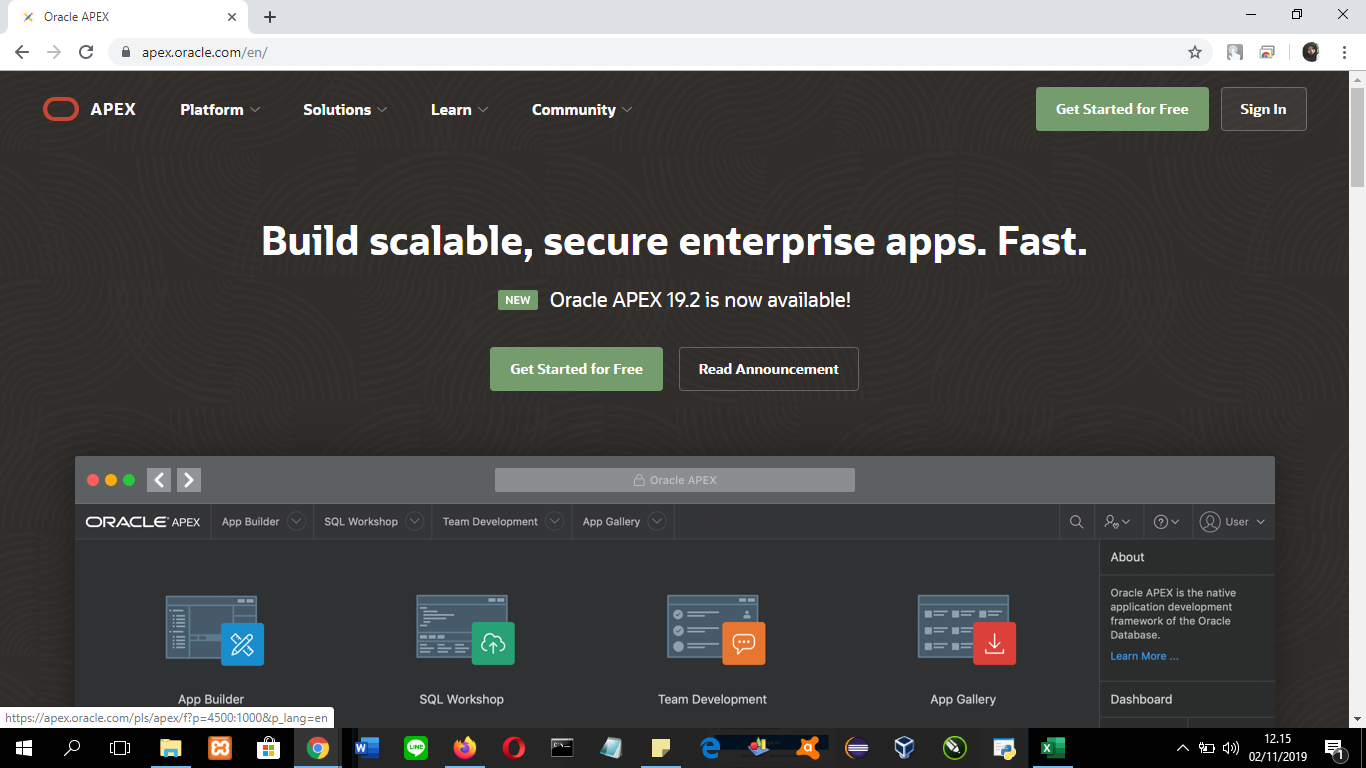
\includegraphics[scale= 0.3]{gambar/gambar1.png}\\
Lalu isi sesuai data kalian\\
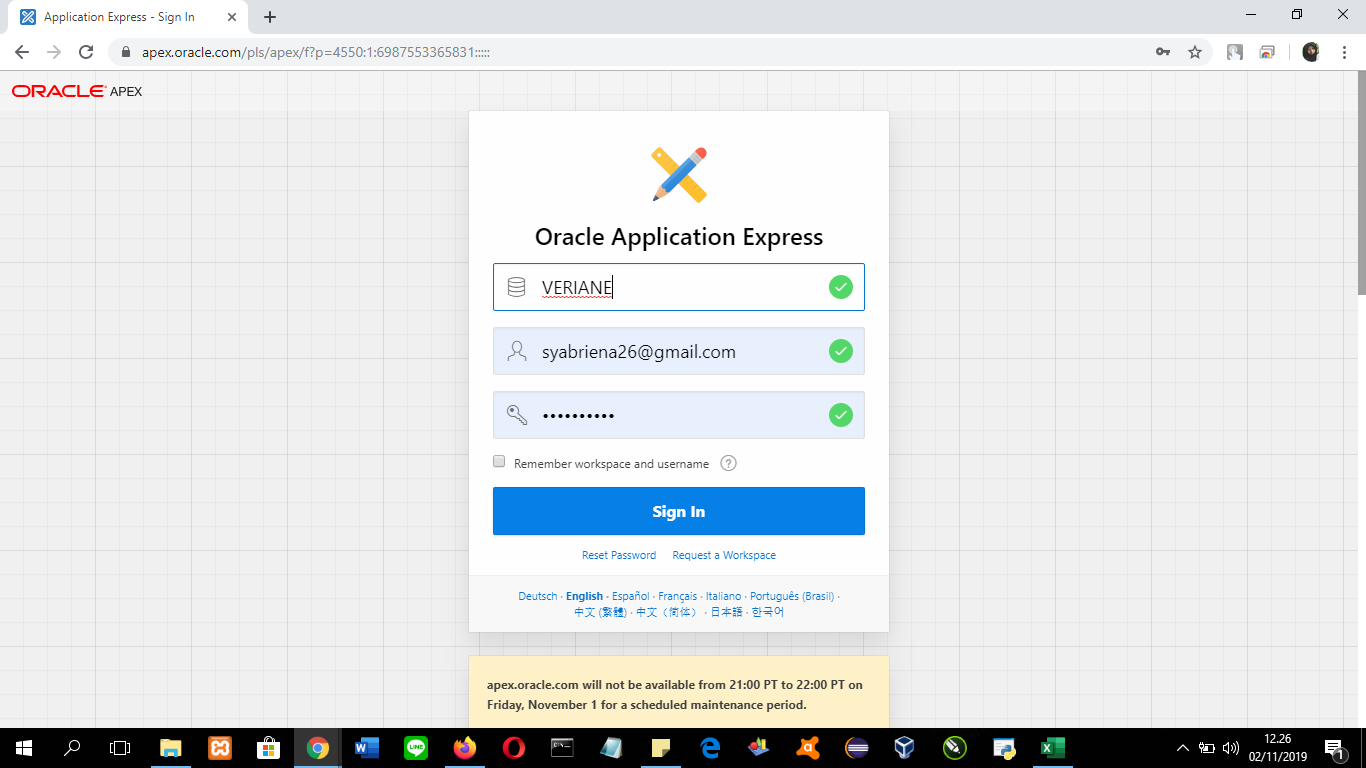
\includegraphics[scale= 0.3]{gambar/gambar4.png}\\

\item Klik App Builder lalu klik Create untuk membuat aplikasi\\
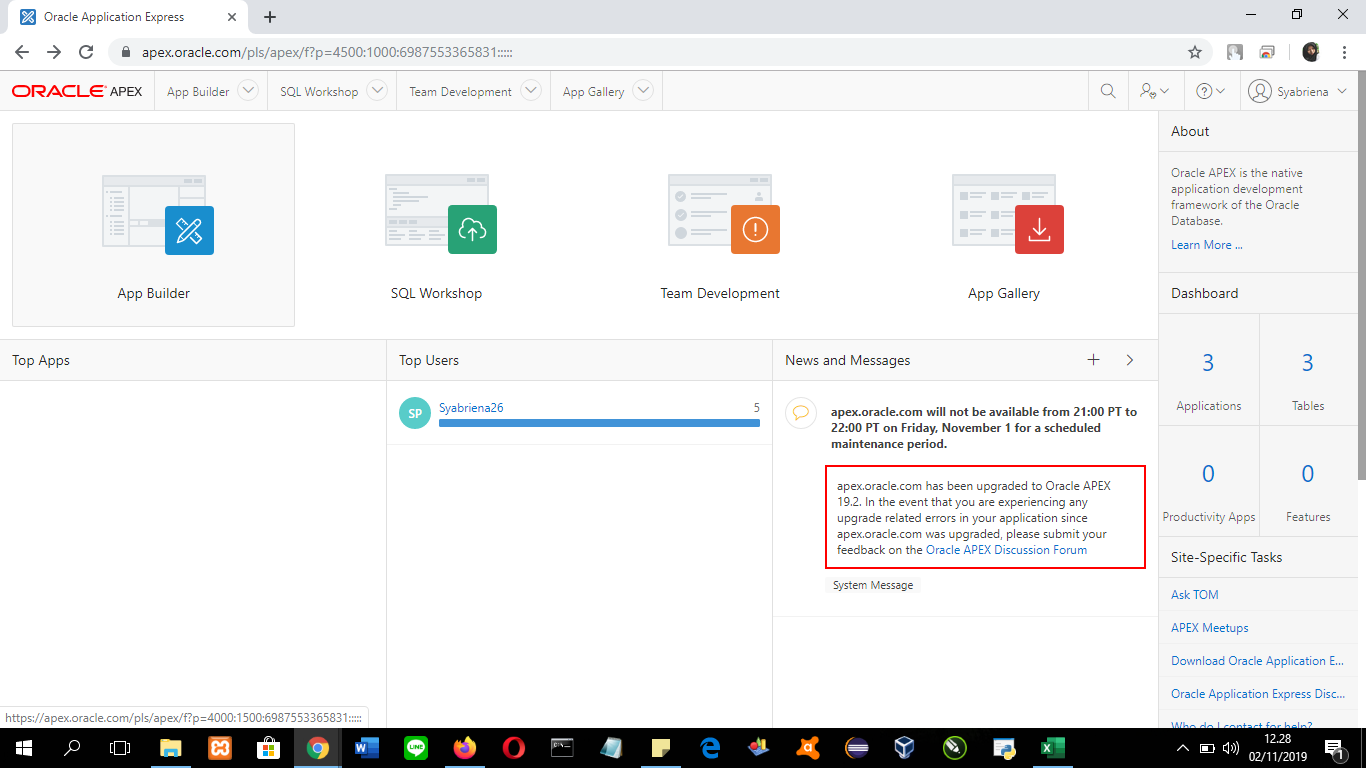
\includegraphics[scale= 0.3]{gambar/gambar5.png}\\
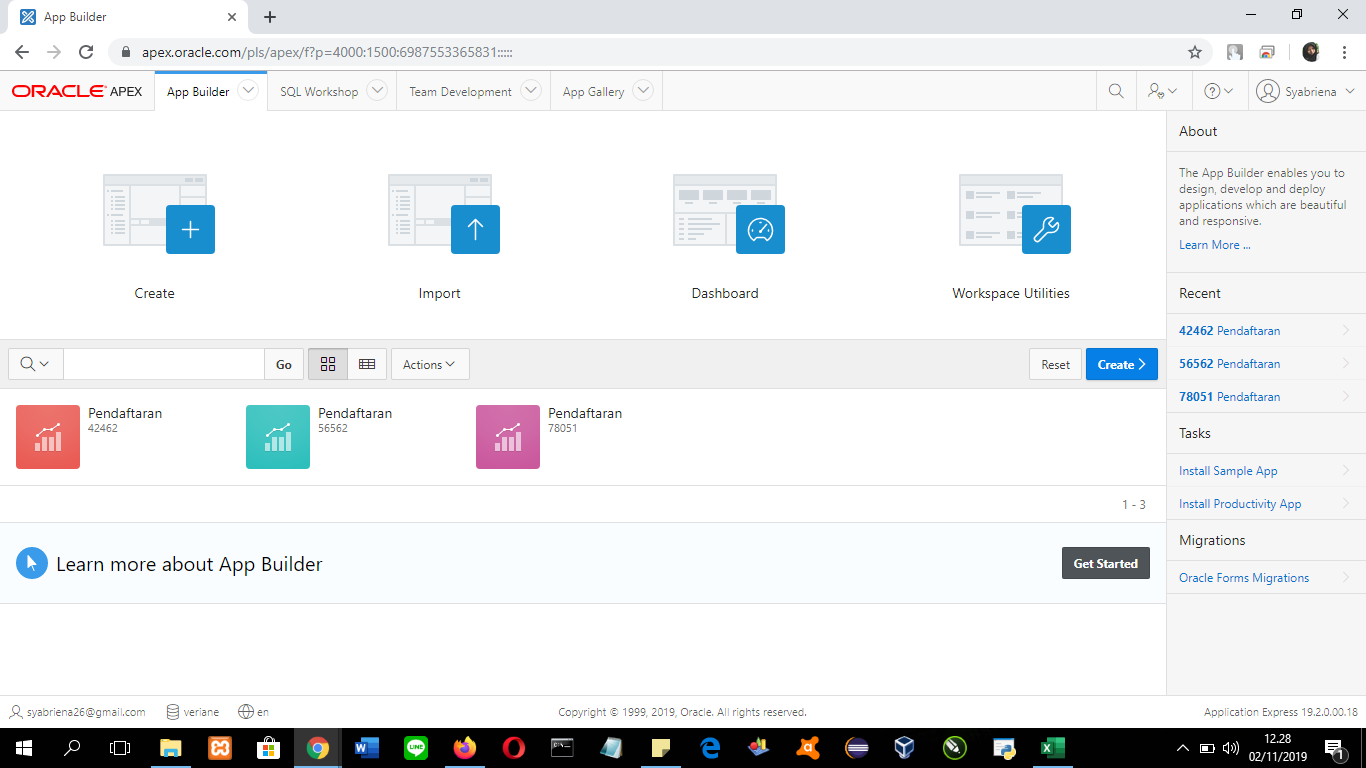
\includegraphics[scale= 0.3]{gambar/gambar6.png}\\

\item Pilih From a file, sebelum itu pastikan kalian sudah memiliki file data csv yang akan dibuat aplikasi\\
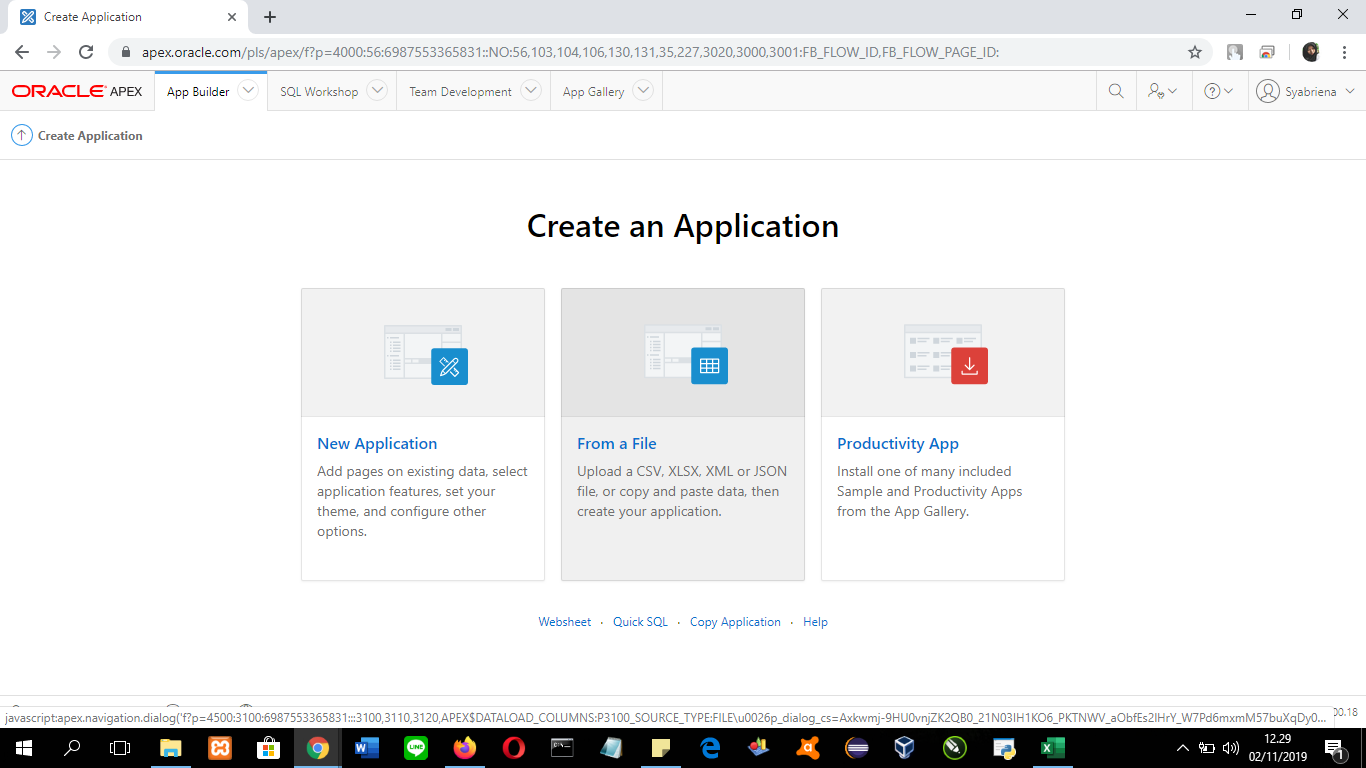
\includegraphics[scale= 0.3]{gambar/gambar7.png}\\

\item Klik Choose file untuk mengupload\\
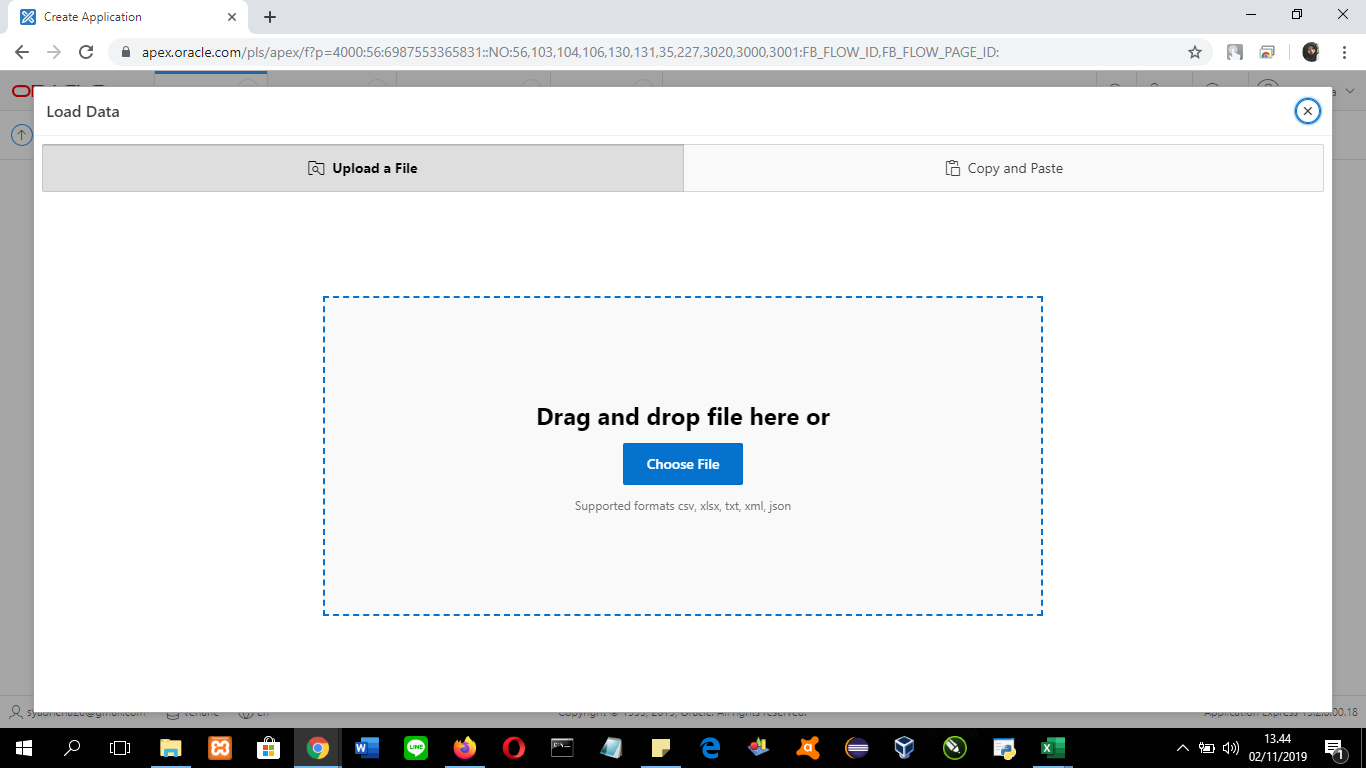
\includegraphics[scale= 0.3]{gambar/gambar8.png}\\
Klik Open\\
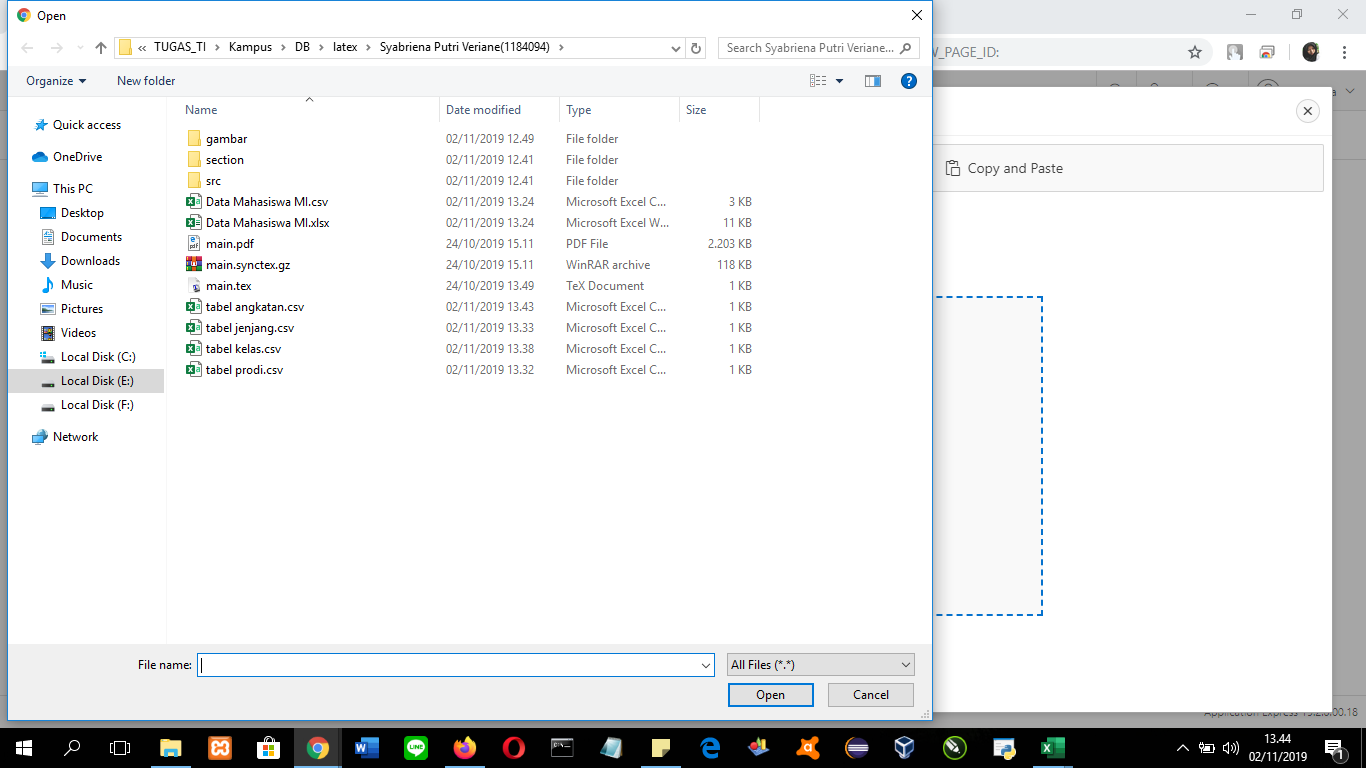
\includegraphics[scale= 0.3]{gambar/gambar9.png}\\
Klik configure\\
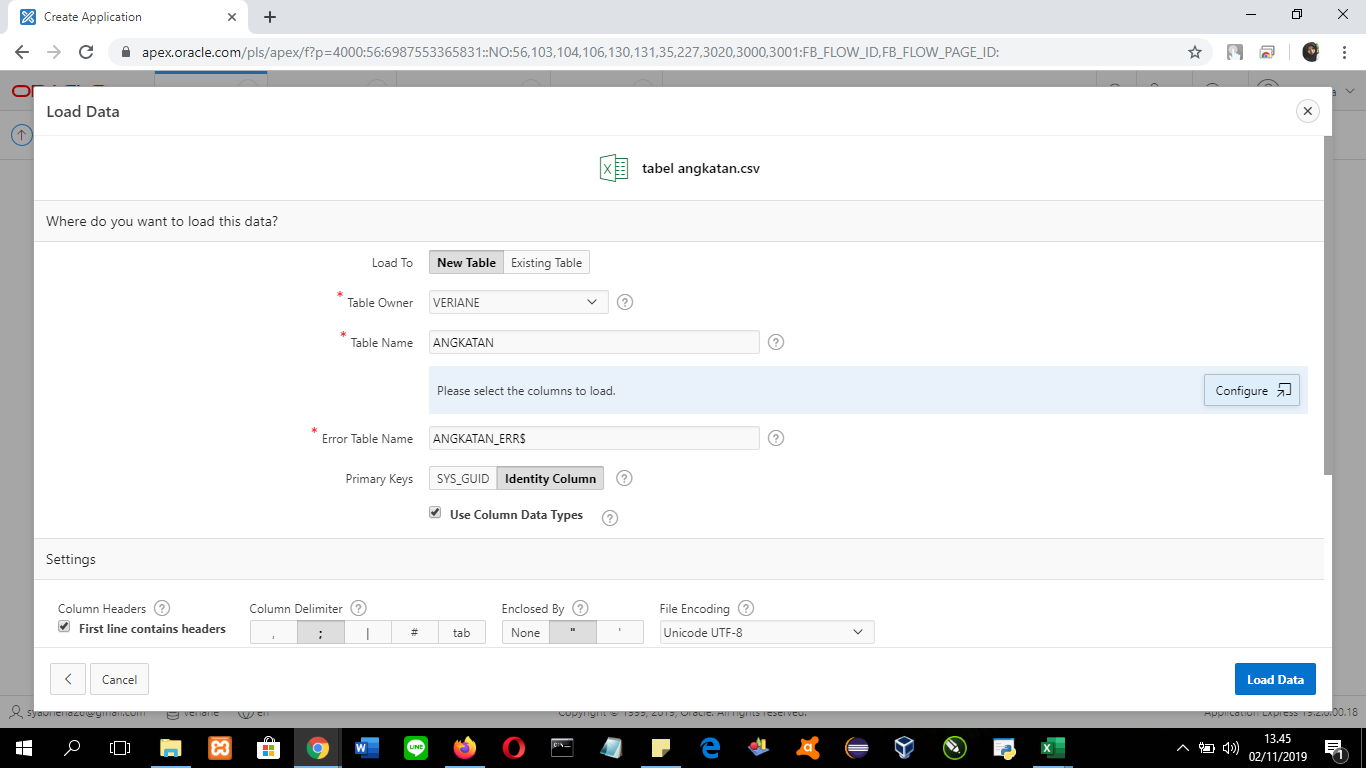
\includegraphics[scale= 0.3]{gambar/gambar10.png}\\
Klik Save changes\\
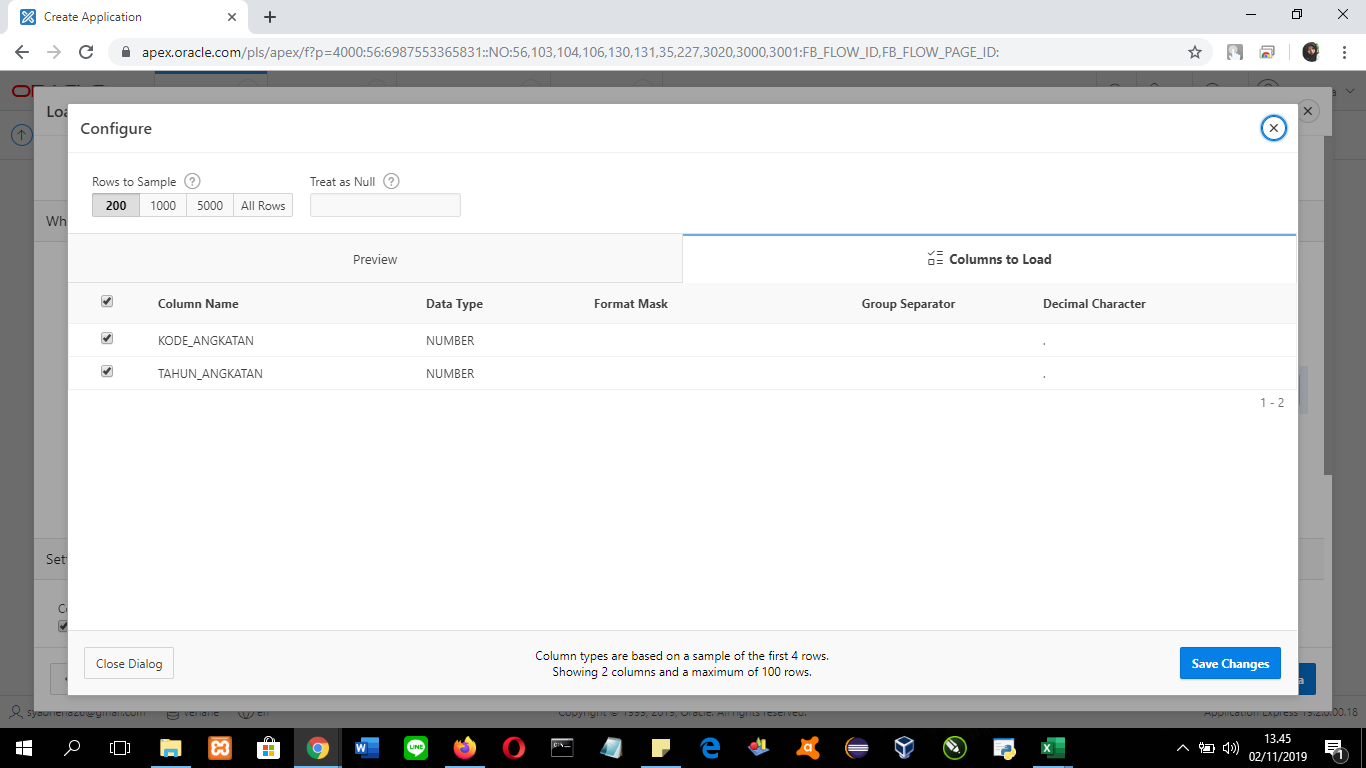
\includegraphics[scale= 0.3]{gambar/gambar11.png}\\
Lalu Klik Load\\
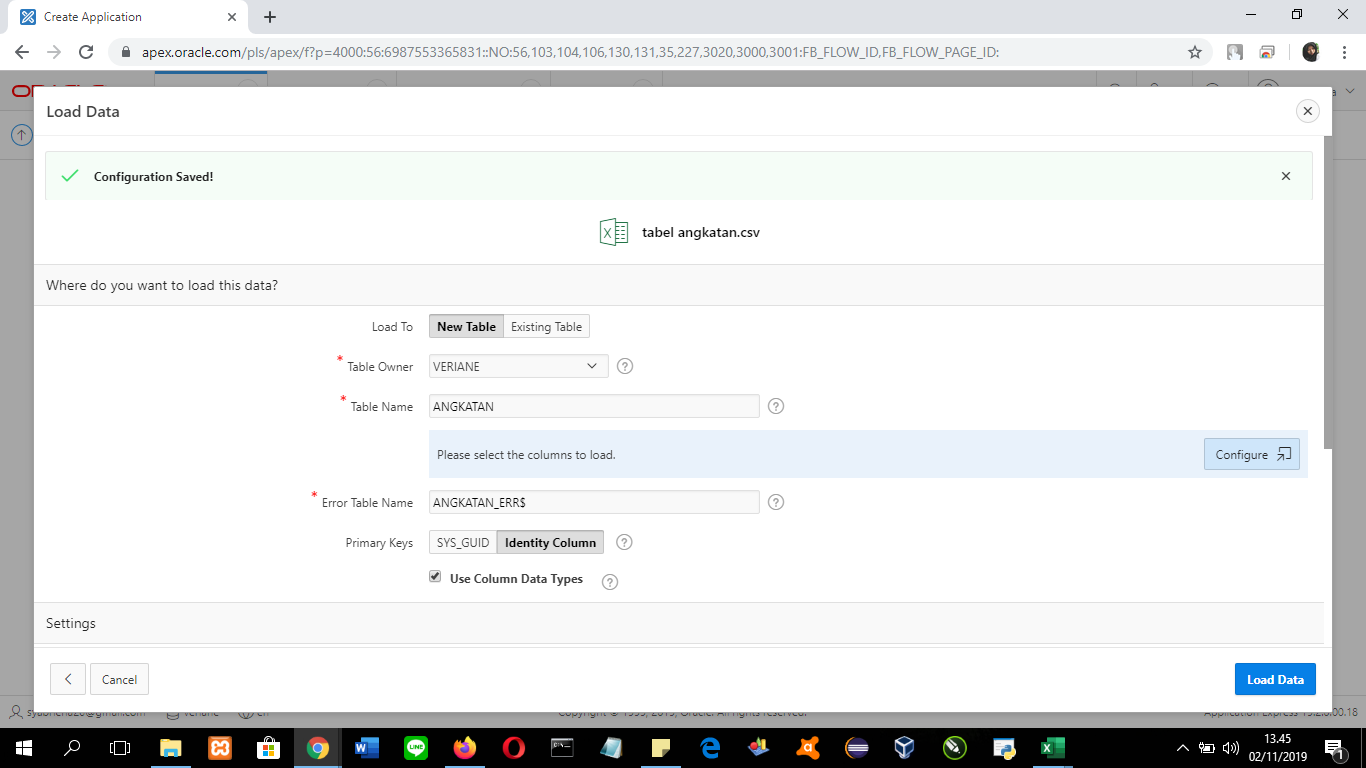
\includegraphics[scale= 0.3]{gambar/gambar12.png}\\
Jika kalian memiliki beberapa file yang akan di upload, setelah load data klik close\\
Setelah di close, lakukan seperti diawal memasukkan file, pastikan yang dimasukkan file yang memiliki size terkecil dahulu.\\
Ketika file size terkecil sudah semua, barulah upload file yang besar\\
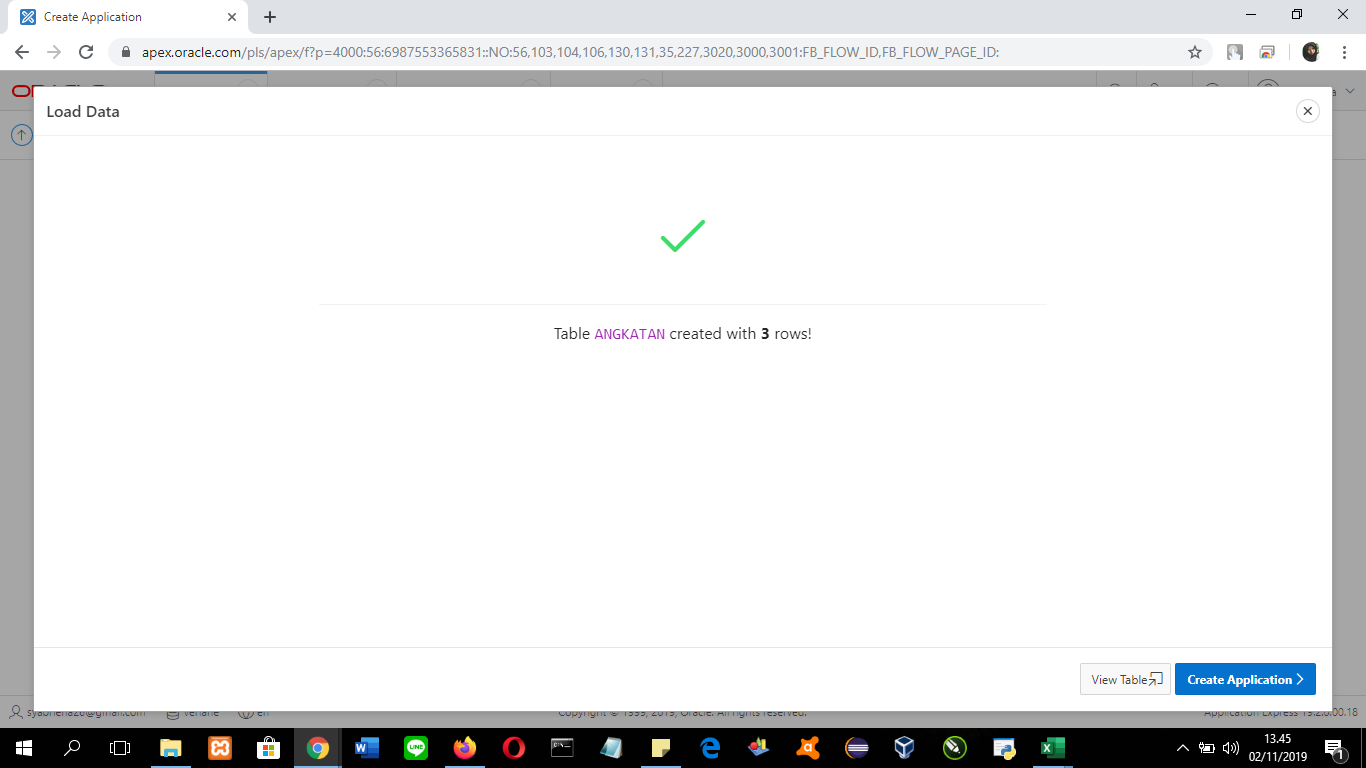
\includegraphics[scale= 0.3]{gambar/gambar13.png}\\

\item Jika semua file sudah di upload, jangan langsung create aplications. Edit dulu semua file, lalu masukkan coding dan coba di run\\
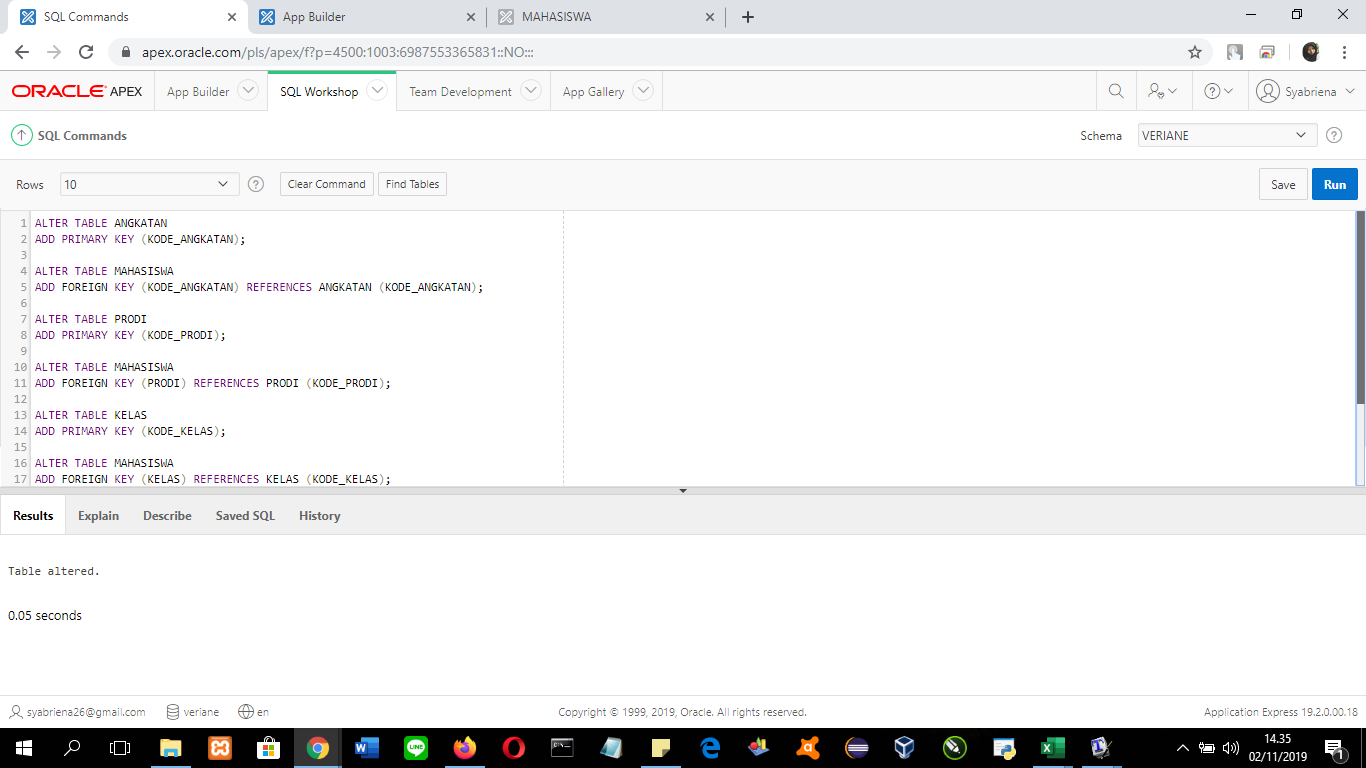
\includegraphics[scale= 0.3]{gambar/gambar17.png}\\

\item Jika semua coding sudah bisa di run dan pastikan tidak ada error, buka app builder kembali lalu create application\\
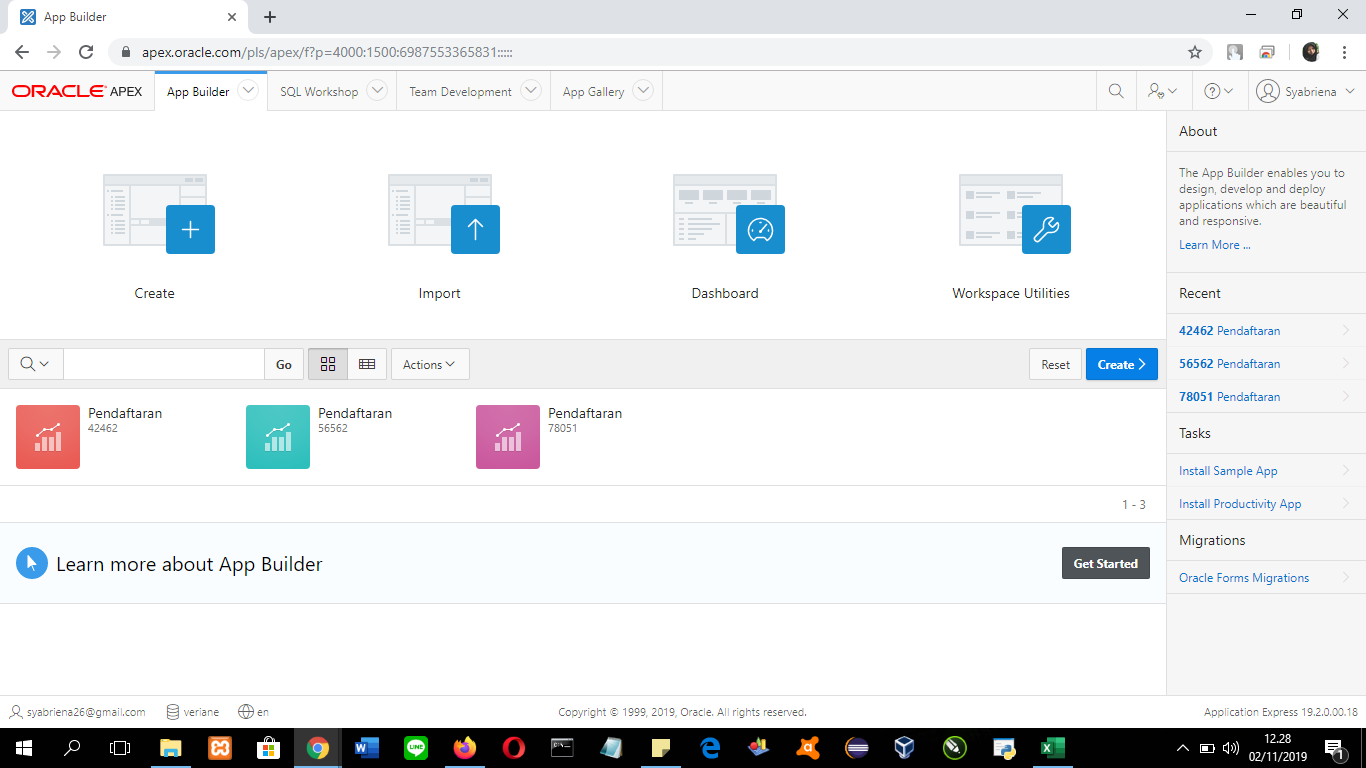
\includegraphics[scale= 0.3]{gambar/gambar6.png}\\

\item Klik new application\\
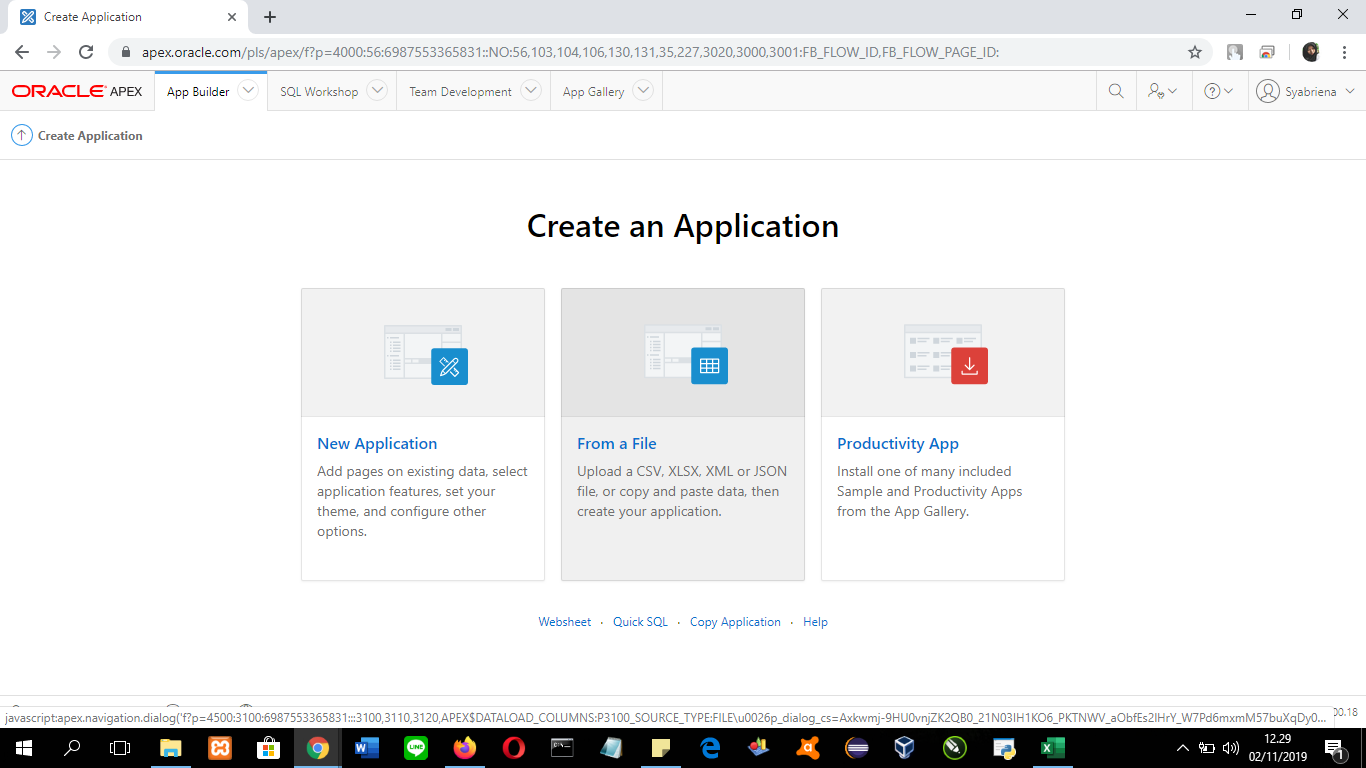
\includegraphics[scale= 0.3]{gambar/gambar7.png}\\

\item Isi nama aplikasi sesuai kehendak kalian\\
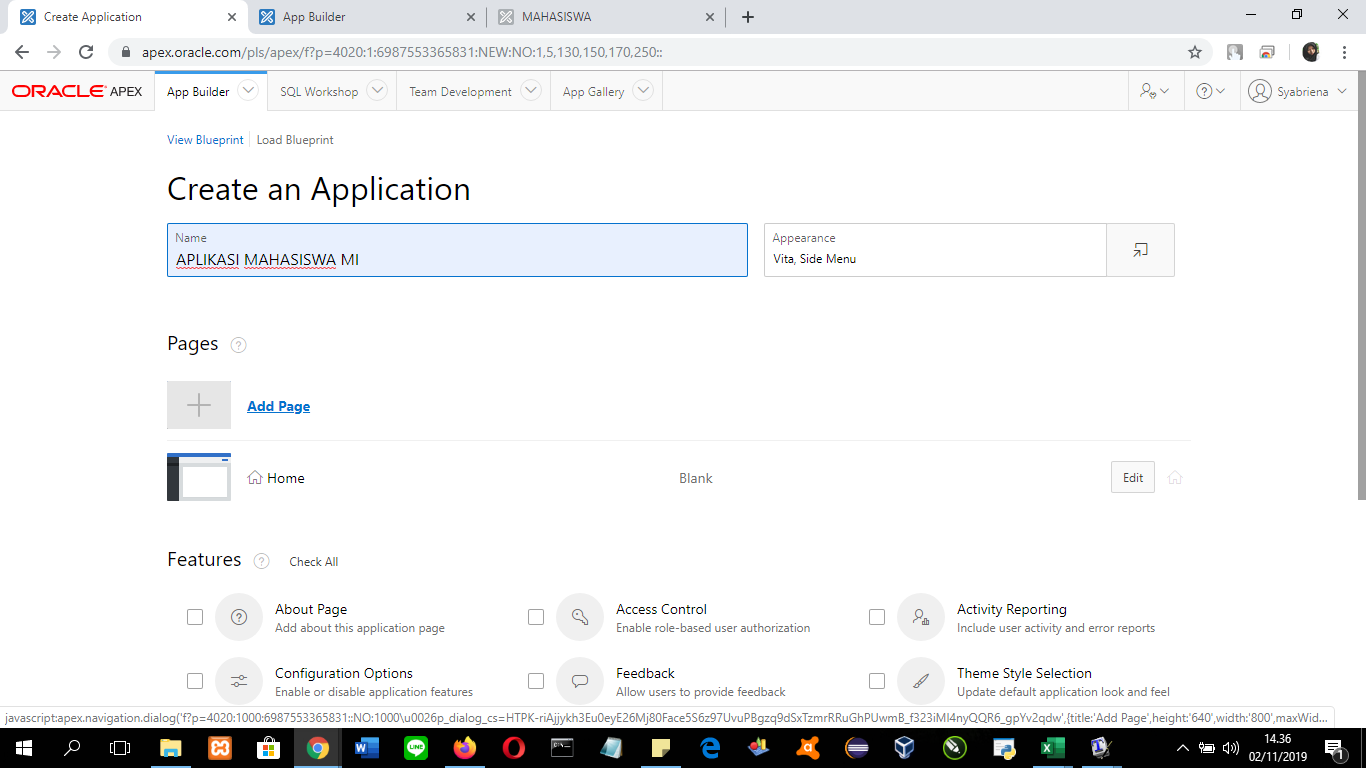
\includegraphics[scale= 0.3]{gambar/gambar18.png}\\

\item Klik Add page, lalu yang pertama klik Faceted Search. Yang kedua klik add page, lalu klik Interactive Report\\
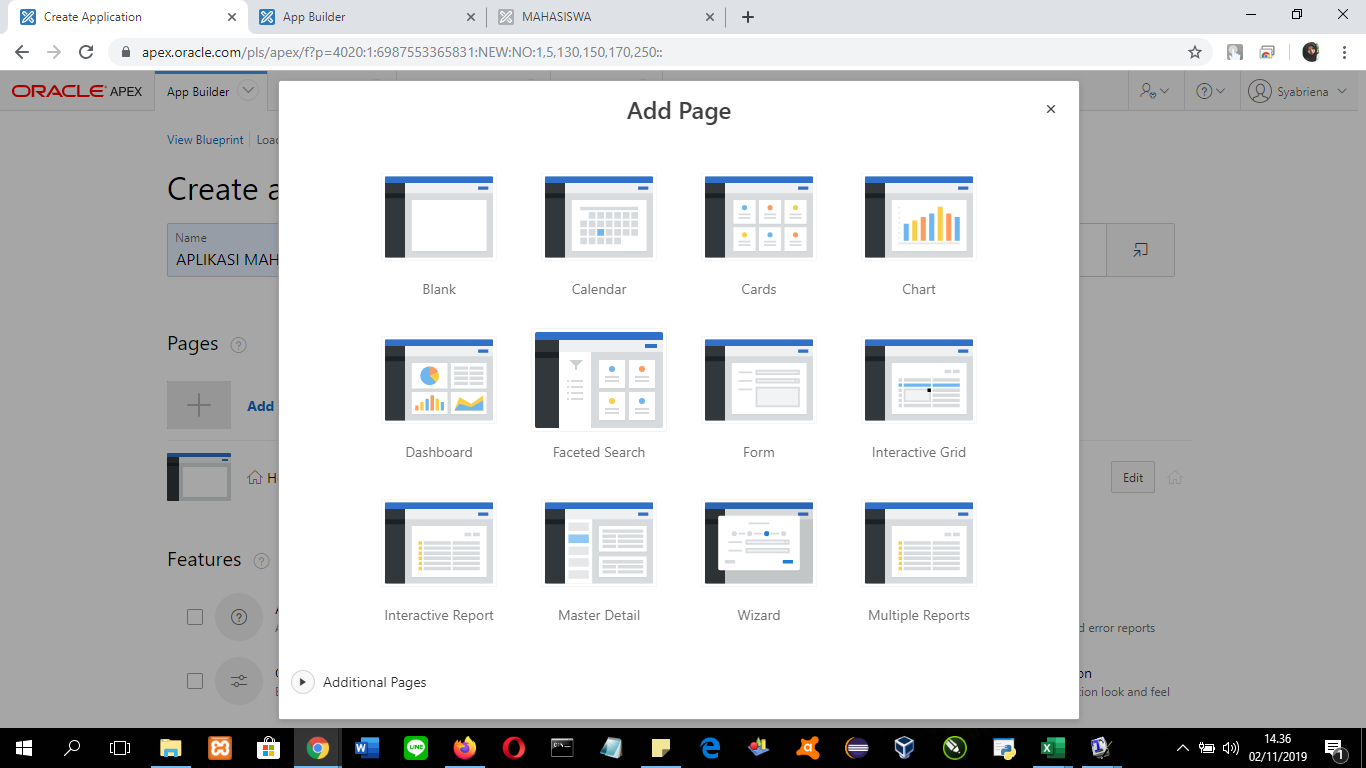
\includegraphics[scale= 0.3]{gambar/gambar19.png}\\
Jika sudah Create Application\\
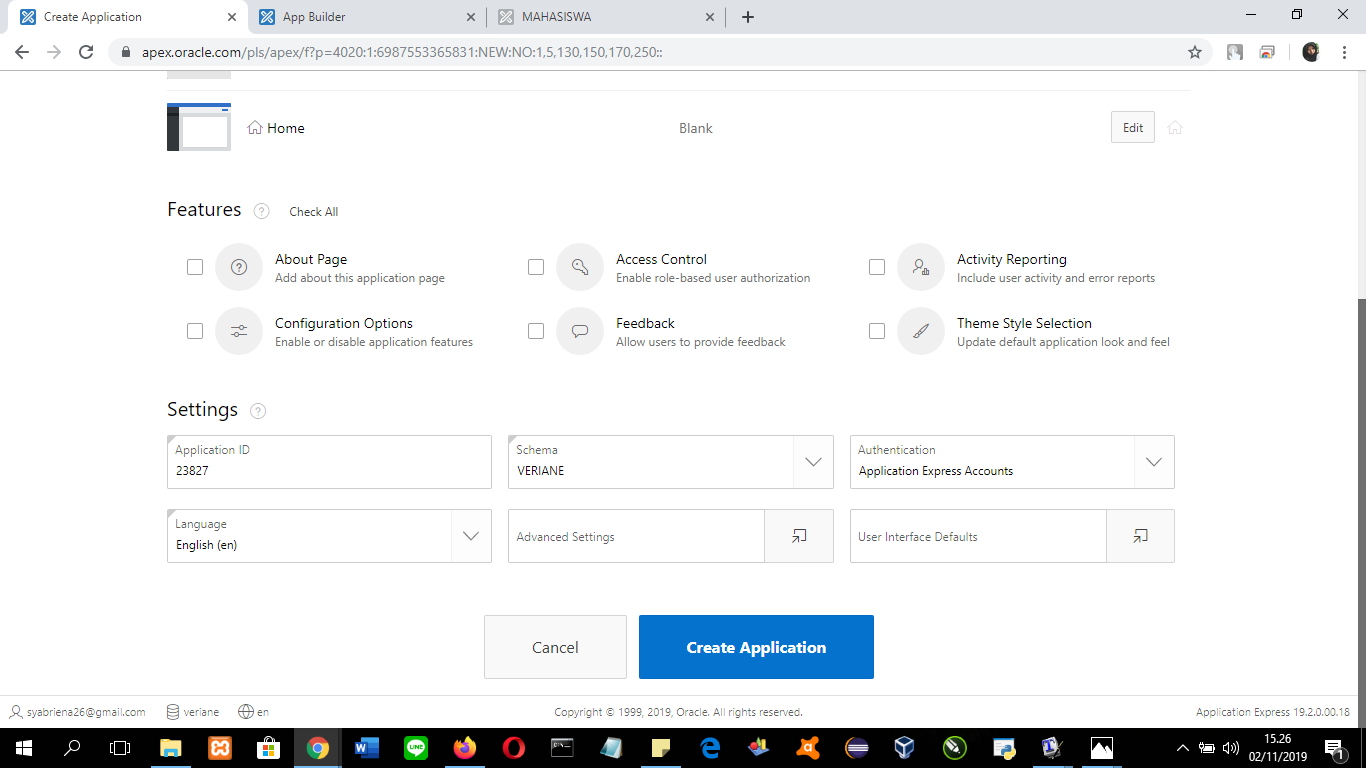
\includegraphics[scale= 0.3]{gambar/gambar20.png}\\

\item Klik Run Application\\
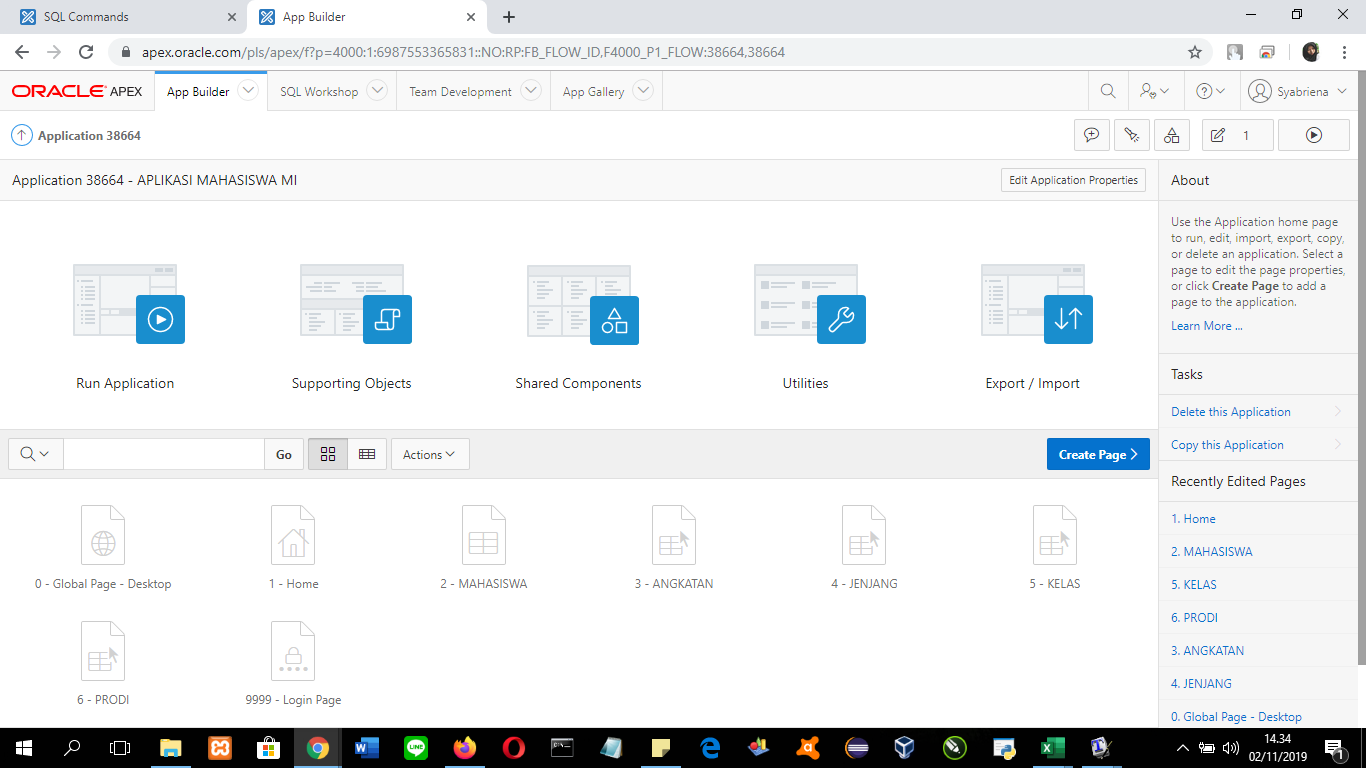
\includegraphics[scale= 0.3]{gambar/gambar14.png}\\

\item Sign in lagi sesuai data kalian\\
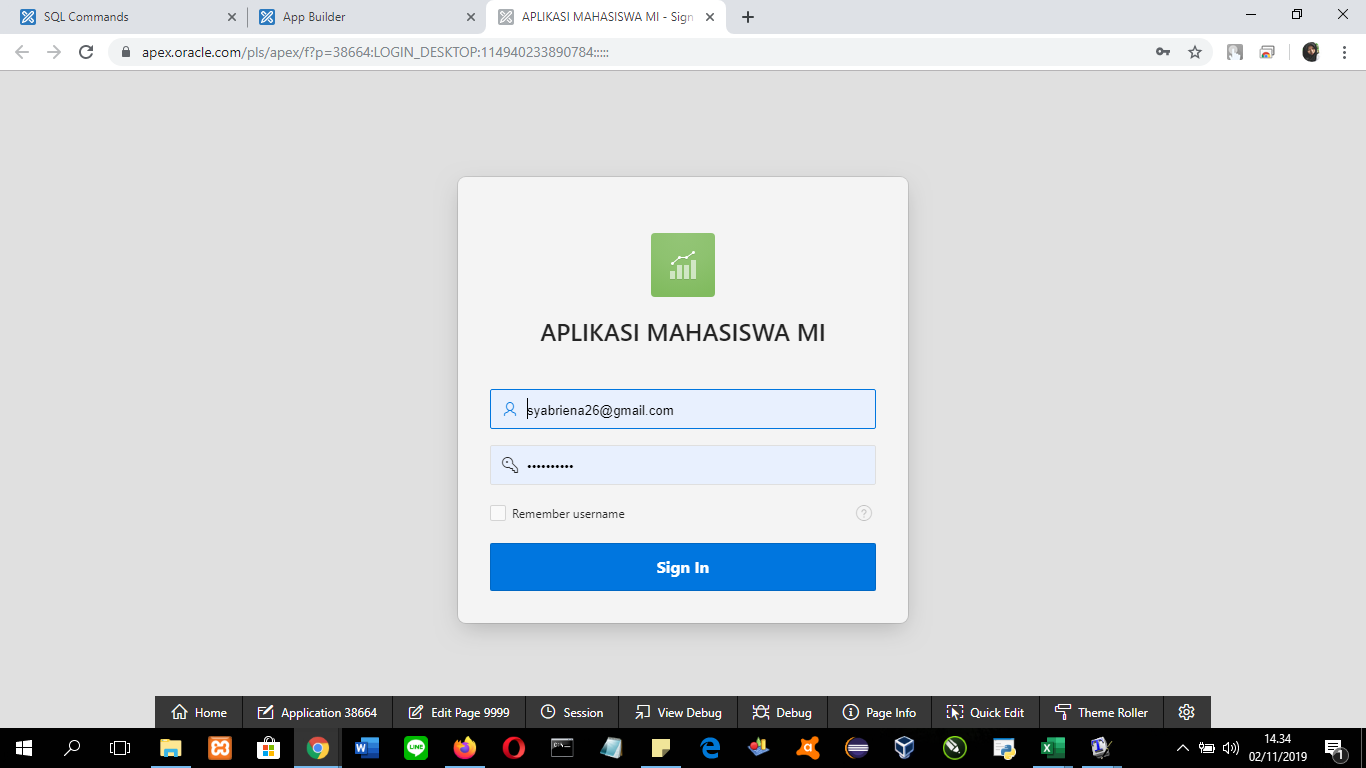
\includegraphics[scale= 0.3]{gambar/gambar15.png}\\

\item Aplikasi sudah jadi.\\
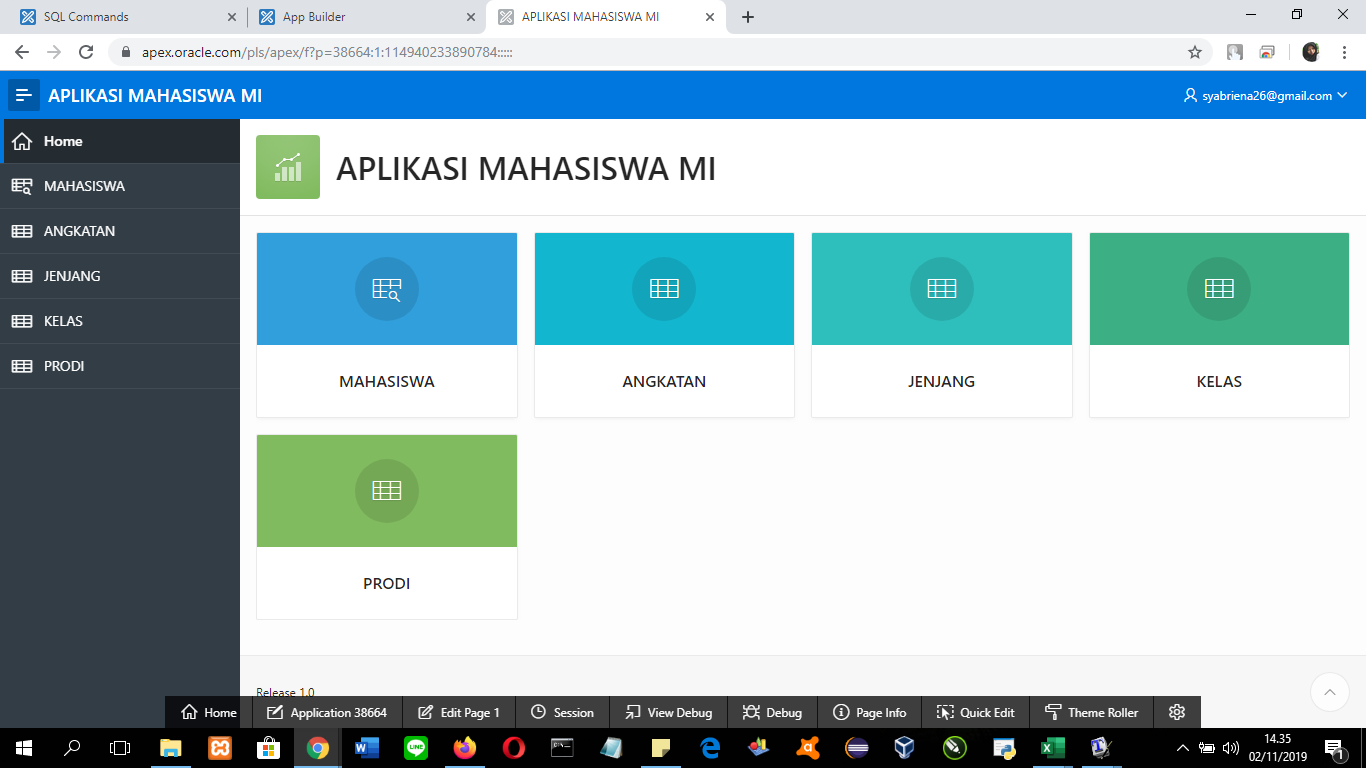
\includegraphics[scale= 0.3]{gambar/gambar16.png}\\
\end{enumerate}

\href{https://apex.oracle.com/pls/apex/f?p=38664:1:114940233890784::NO:::}{LINK APLIKASI}